\section{Known Limitations}
\label{sec:limitations}

\subsection{SPI Register Addressing Off-by-One Error}
\label{subsec:spi_register_offset}
As illustrated in \autoref{tab:reg_des}, register two is absent. This absence was not intentional but a consequence of historical developments. Initially, registers one and two were designed as read-only registers to provide status information about the chip, such as an over-temperature fault condition. However, it was later on decided not to implement these functionalities. Consequently, one register was eliminated, and a constant value was assigned to the remaining one (Register 1), as shown in \autoref{tab:reg_des}.
This modification was made a few weeks prior to the tape-out, and as a result to a tight timeline it was overlooked that the test bench and address mapping of the design must be updated to reflect this change. Therefore, to write to the first write register, the access must address register three instead of register two, as register two does not exist. While this is limitation does not impede functionality, it is an important consideration when accessing the registers.

\subsection{Current Measurement Inaccurate if $V_{DDL} \neq V_{IN}$}
\label{subsubsec:cur_mes_inac}
The internal inductor current $I_L$ measurement circuitry operates on the principle, that it amplifies the voltage drop over the input \ac{PMOS} transistor. This approach works as the voltage drop during conduction can be approximated as 
\begin{equation}
    V_{DS,on} = R_{DS,on} \cdot I_L
\end{equation}
\label{eq:Vds}
leading to 
\begin{equation}
    I_L \approx \frac{V_{DS,on}}{R_{DS,on}}
\end{equation}
\label{eq:IL}
As $R_{DS,on}$ is a known quantity and $V_{DS,on}$ can be directly measured, this approach can be used to measure the current flowing through the transistor.
The on-resistance of the transistor is thus used as a current measurement shunt resistor. \autoref{eq:IL} however only holds if the transistor is conducting current and thus the amplifier output is only valid in this case. In the non-conducting phase, the circuit would ordinarily still amplify the large voltage differential between source and drain leading to an output corresponding to a large inductor current. To combat this, we implemented a circuit to short the amplifier inputs when the input transistor is non-conducting, leading to an output corresponding to no inductor current. As the regulator implements peak-current mode control, the 0 current reading in the non-conducting phase leads to no problems and allows the circuit to start in the correct operating point when conduction starts. \\
In the implementation of the circuit we mistakenly shorted the inverting amplifier input $V_M$ with the logic supply $V_{DDL}$ instead of the converter power input $V_{IN}$, which is connected to the non-inverting amplifier input $V_P$ as can be seen in \autoref{fig:currentmeas}. In the simulation where $V_{DDL} = V_{IN}$ was always ued, this poses no problems as it does in practice when these conditions are applied. In cases where $V_{DDL} = V_{IN}$ is not applicable, the current measurement in the non-conducting phase generates an inaccurate current reading of large magnitude. This applies to cases where $V_{DDL} \neq V_{IN}$ is a static condition, e.g. $V_{DDL} = \qty{5}{\volt}; V_{IN}= \qty{4.3}{\volt}$, as well as for dynamic conditions such as when $V_{DDL} = V_{IN}$ set, but large current transient cause a voltage drop on $V_{VIN}$.\\
This issue could have various knock-on effects like the discontinuous regulation observed in \autoref{sec:loadRegulation} but we could not prove this conclusively. The described issue could also exacerbate the issues with the start-up behavior as the large input current during start-up could lead to a voltage differential between $V_{DDL}$ and $V_{IN}$ causing issues in the current readings. A compounding issue is that any voltage transients get differently attenuated by the off-chip bypassing on both power-rails leading to unmeasurable dynamic errors in the current measurement.

\begin{figure}[h]
    \centering
    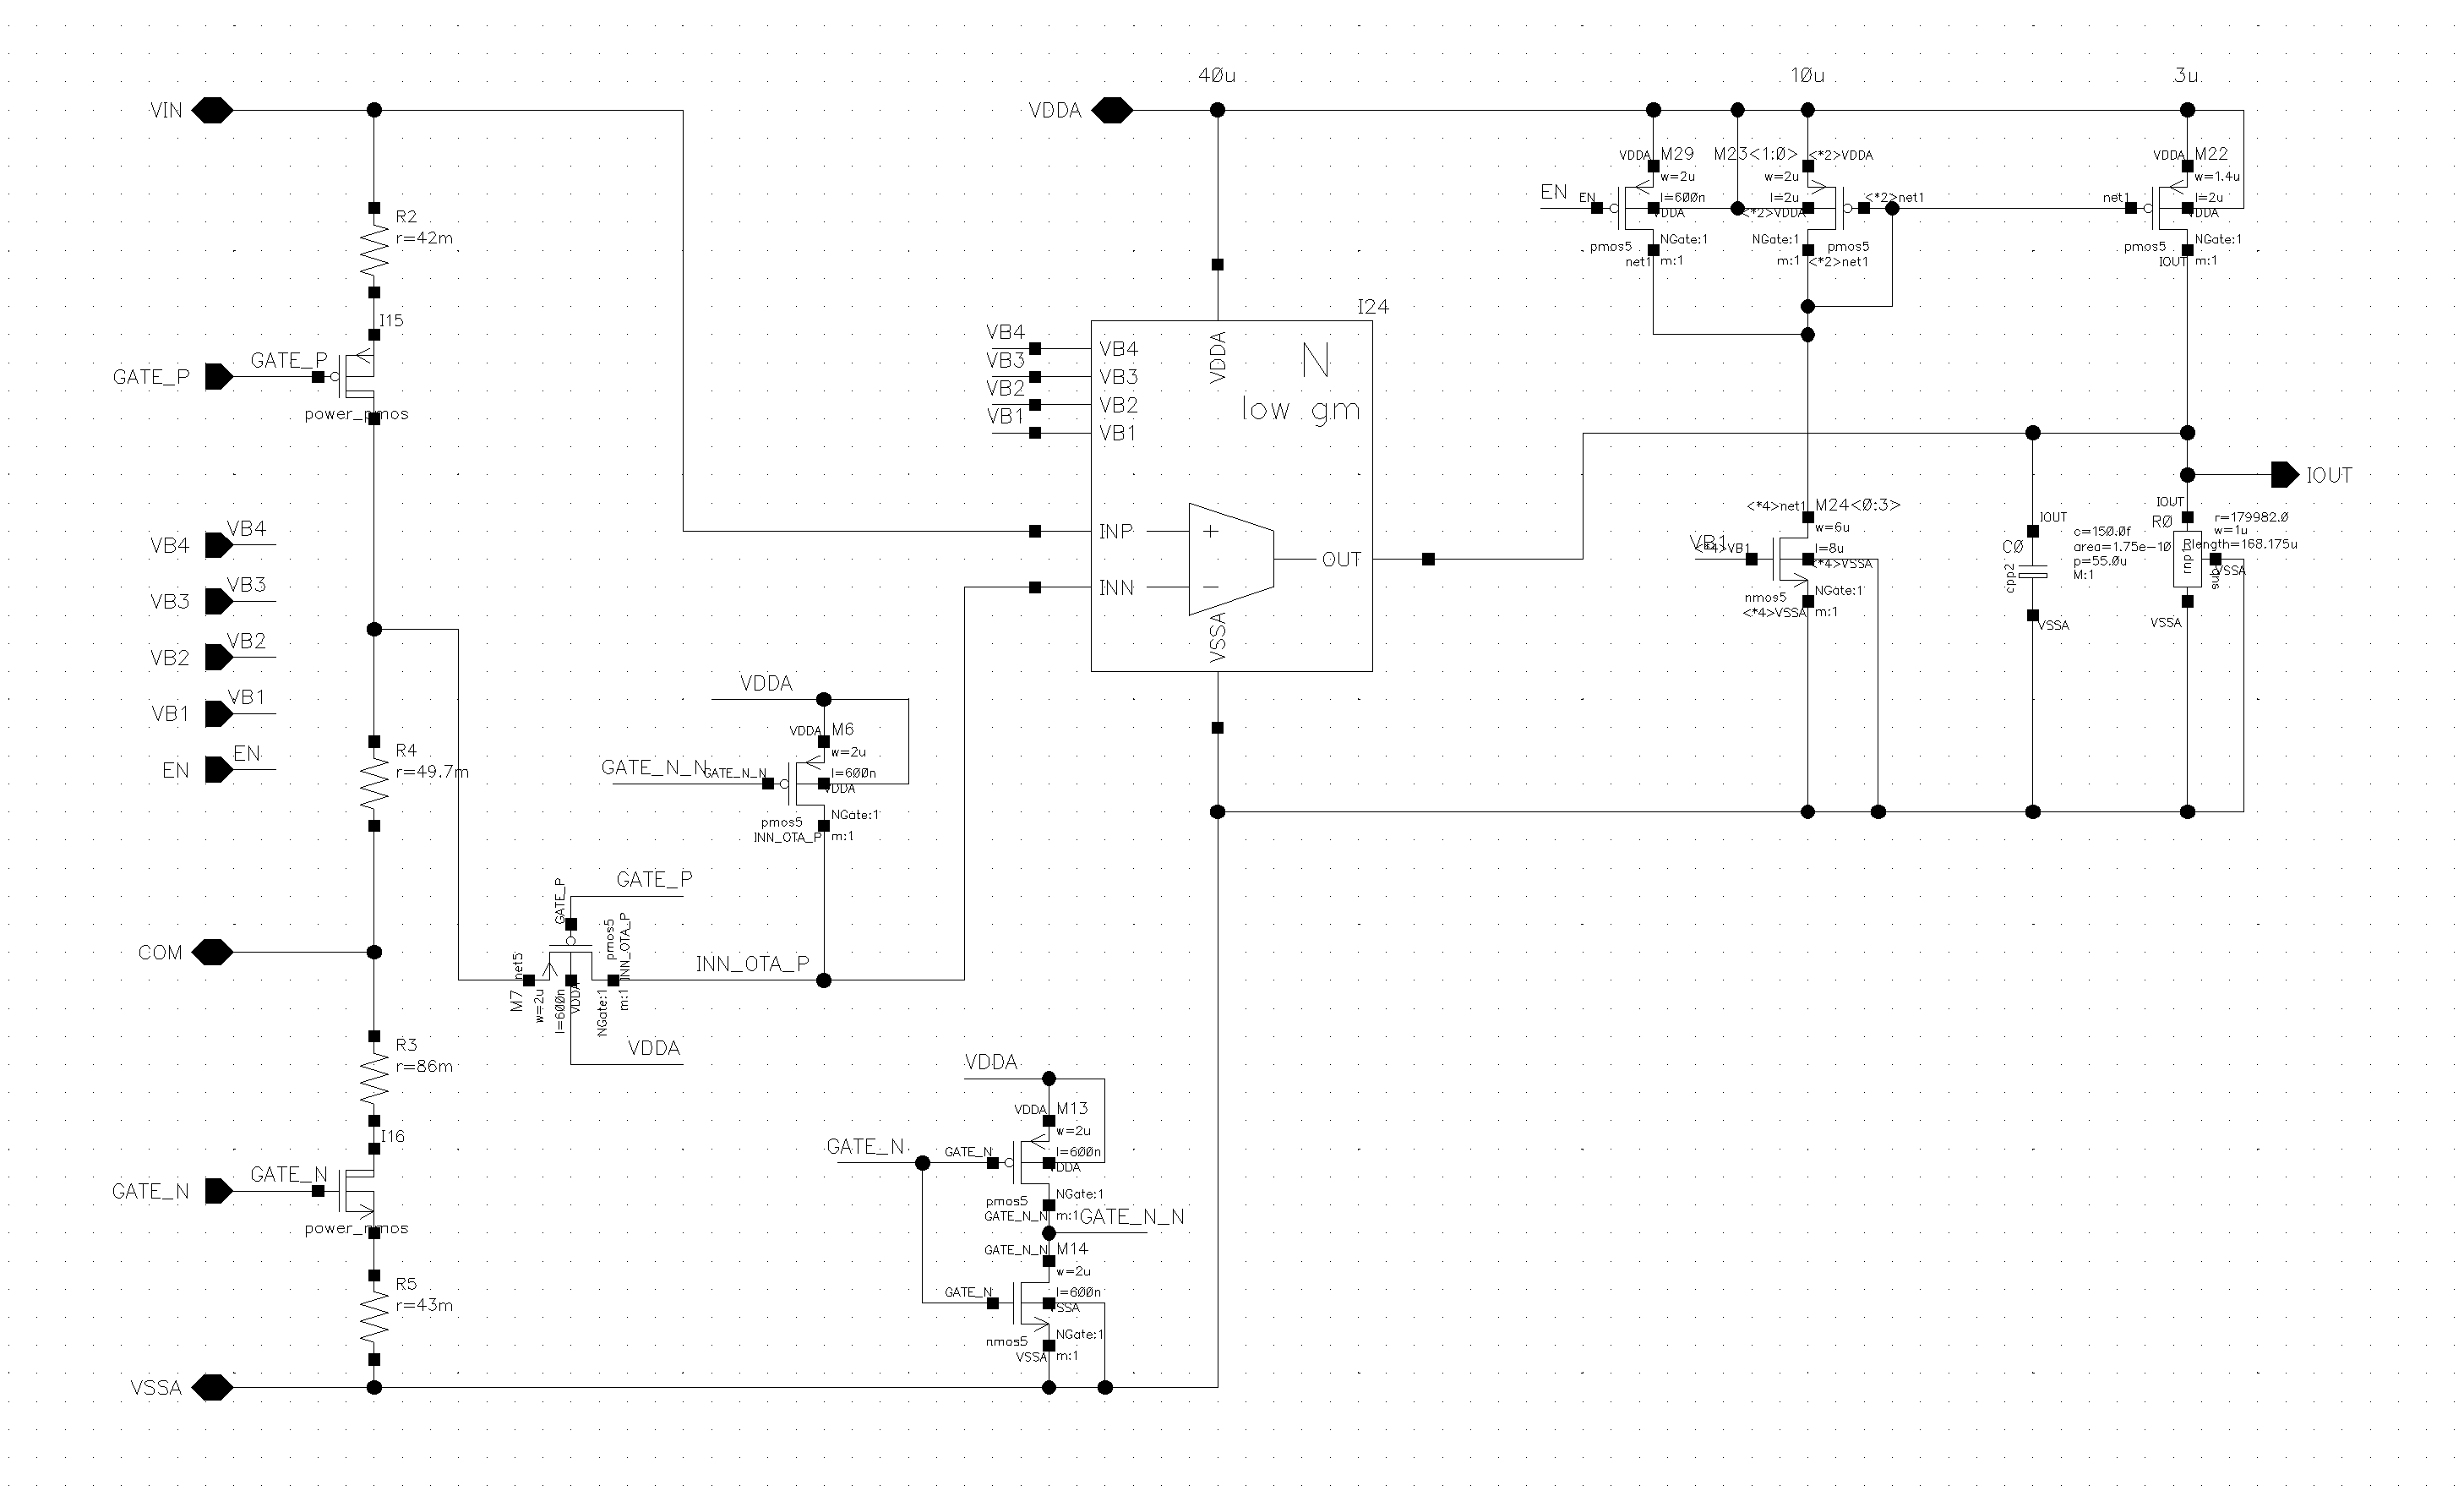
\includegraphics[width=1\textwidth]{../ASIC-DESIGN-2/images/07_DCDC/CurrentMeas.png}
    \caption{Current measurement circuit with the error of connecting the source of M6 with VDDL (VDDA in this figure) instead of VIN}
    \label{fig:currentmeas}
\end{figure}


\subsection{Default Register Settings Disables Current Limit}
\label{sec:missingcurrentlimit}

A misconfiguration of the default state in the internal registers causes the current limit for the converter to be disabled at start-up. This causes the converter to start operating without an effective current limit leading to the converter pulling excessive amounts current at start-up, leading the supply to collapse to under the limit set by the \ac{POR}. This behavior is documented in \autoref{sec:startup}. The current limit can be enabled after start-up and works as intended, but as the settings are stored in non-persistent memory, they are lost after restart and the chip therefore cannot begin operation with the current limit enabled. 
\clearpage

\subsection{Internal Current Reference Out of Specification}
During testing, the internal current reference of the ASIC was discovered to be out of specification. The measured current was approximately \qty{4}{\micro\ampere} higher than the simulated value, representing a deviation of about 38.8\%. While an exact cause for this discrepancy was not identified, it is hypothesized that the deviation may be attributable to the resistors used in the layout of the current reference.

The current reference plays a pivotal role in the \ac{ASIC}, providing a stable reference current for various circuit components. Consequently, any deviation in the current reference can significantly affect the overall performance of the \ac{ASIC}. Despite this, apart from some increased current consumption, the other blocks appeared to function as expected, even with the elevated current. However, the impact of the higher current is noticeable in certain blocks, such as the bandgap circuit. In the simulation, the voltage peaks over temperature is at \qty{40}{\degreeCelsius}, but in the measurement with the higher current, it peaks at approximately \qty{55}{\degreeCelsius}, as also discussed in \autoref{subsubsec:bandgap}.

For more details on the current reference, please refer to \autoref{subsubsec:current_source} and the corresponding figures.

\subsection{Internal Oscillator Out of Specification}
The internal oscillator of the \ac{ASIC} was also found to be out of specification during testing. The measured frequency was significantly higher than the simulated value, resulting in a deviation of approximately 54.7\% as it can be seen in \autoref{subsubsec:oscillator}. Since this circuits frequency is not dependent on the current reference, but only on the bandgap voltage, the absolute value of an rnp1 resistor and MIM-capacitors, we find the resistor is the most likely issue. 
